% Group 10 - progress report (70-80% milestone), Information Retrieval.
% Build: pdflatex 10_BM25NeuralRetrieval.tex (twice). Self-contained: every number below was checked
% against the committed result files (see README.md in this folder for the sources).
\documentclass[10pt,a4paper]{article}
\usepackage[margin=1.7cm,top=1.4cm,bottom=1.6cm]{geometry}
\usepackage[T1]{fontenc}
\IfFileExists{lmodern.sty}{\usepackage{lmodern}}{\usepackage{mathptmx}}
\IfFileExists{lmodern.sty}{}{\usepackage{courier}}   % vector monospace font (avoids bitmap Type 3 fonts)
\usepackage{microtype,booktabs,xcolor,tabularx,amsmath,enumitem,array}
\usepackage[font=small,labelfont=bf,skip=3pt]{caption}
\usepackage{float}
\usepackage{tikz}
\usetikzlibrary{positioning,arrows.meta,fit,backgrounds,calc}
\usepackage[colorlinks,urlcolor=blue!60!black,linkcolor=black,citecolor=black]{hyperref}
\setlist{nosep,leftmargin=1.2em}
\setlength{\parskip}{2.5pt}
\setlength{\parindent}{0pt}
\setlength{\textfloatsep}{8pt}
\setlength{\floatsep}{6pt}
\setlength{\intextsep}{6pt}
\renewcommand{\arraystretch}{1.08}
\newcommand{\repo}{\url{https://github.com/surajsinhpatil/bm25-vs-neural}}
\newcommand{\done}{\textcolor{green!45!black}{\textbf{done}}}
\newcommand{\todo}{\textcolor{orange!80!black}{\textbf{remaining}}}
\newcommand{\sect}[1]{\vspace{2pt}\section{#1}\vspace{-2pt}}

\begin{document}
% ===================================================================================== page 1
\begin{center}
{\Large\bfseries Domain-Specific Search: BM25 vs.\ Neural Retrieval on Technical Documents}\\[3pt]
{\large Progress Report (70--80\% milestone) \;|\; Information Retrieval \;|\; Group 10}\\[5pt]
\begin{tabular}{@{}llcll@{}}
Surajsinh Patil & 2025H1030058P & \hspace{2em} & Tejas Mahajan & 2025H1030057P\\
Swayam Kumud & 2025H1030063P & & Saksham Singhal & 2025H1030208P
\end{tabular}\\[4pt]
\textbf{GitHub repository:} \repo
\end{center}

\textbf{Objective.} Dense retrievers are often assumed to have made BM25 obsolete. We test this on technical
text, where relevance depends on exact strings (CVE numbers, protocol versions) as well as on paraphrase:
39{,}613 arXiv computer-security (cs.CR) abstracts and 50 queries in five categories (exact identifier,
homonym, negation, time constraint, paraphrase). We compare our own identifier-aware BM25 with two dense
retrievers used without fine-tuning (E5-base-v2, SPECTER2) and their Reciprocal Rank Fusion (RRF) hybrids,
on graded relevance judgments that we collected ourselves. Research questions: \textbf{RQ1} does a dense
retriever beat BM25? \textbf{RQ2} how does this depend on the query type? \textbf{RQ3} does the
science-specific SPECTER2 beat the general E5? \textbf{RQ4} does a hybrid beat both of its components?
\textbf{RQ5} how sensitive is BM25 to $k_1$, $b$ and tokenisation?

\textbf{Progress.} The full pipeline is implemented, tested (81 unit and end-to-end tests) and has been run on
the real corpus. All five research questions have results on frozen, double-judged, adjudicated relevance
judgments. We estimate that roughly three quarters of the planned work is complete. What remains
(Section~\ref{sec:plan}) is a second blind judging round for documents that the stretch-objective and RQ5 runs
retrieve but nobody has judged yet, the evaluation of the stretch objectives that depends on it, and the
final report and demonstration.

\sect{Implementation status and architecture}
\begin{table}[H]\centering\small
\caption{Implementation status (all components are in the repository).}\label{tab:status}
\begin{tabularx}{\linewidth}{@{}l l X@{}}
\toprule
Component & Status & Evidence\\
\midrule
Corpus builder, frozen corpus & \done & 39{,}613 docs, SHA-256 \texttt{fda391ecc5b6\ldots}, arXiv id list committed\\
Identifier-aware tokeniser + BM25 (own code) & \done & matches Lucene/Pyserini on BEIR SciFact ($\Delta$nDCG@10 $=-0.0009$)\\
Dense retrieval (E5, SPECTER2), RRF hybrids & \done & five TREC runs, GPU encoding on Kaggle, exact cosine search\\
Pooling, blind double judging, adjudication & \done & 1{,}339 pairs, 2{,}678 judgments, weighted $\kappa=0.76$, frozen qrels + provenance\\
Metrics, significance, efficiency, error analysis & \done & metric code equals \texttt{trec\_eval}; randomisation tests with Holm correction\\
RQ5: $k_1$/$b$ sweep and tokenisation ablation & \done{} (exploratory) & 132 settings, 5 analyzers, run on Kaggle with corpus and qrels checks\\
Stretch S1 (cross-encoder), S2 (date filter) & runs done, \todo & their new top-10 documents (157 pairs) are unjudged\\
Stretch S3 (LLM judge), S4 (score fusion) & code done, \todo & tested on synthetic data; not yet run on cs.CR\\
\bottomrule
\end{tabularx}
\end{table}

\begin{figure}[H]\centering
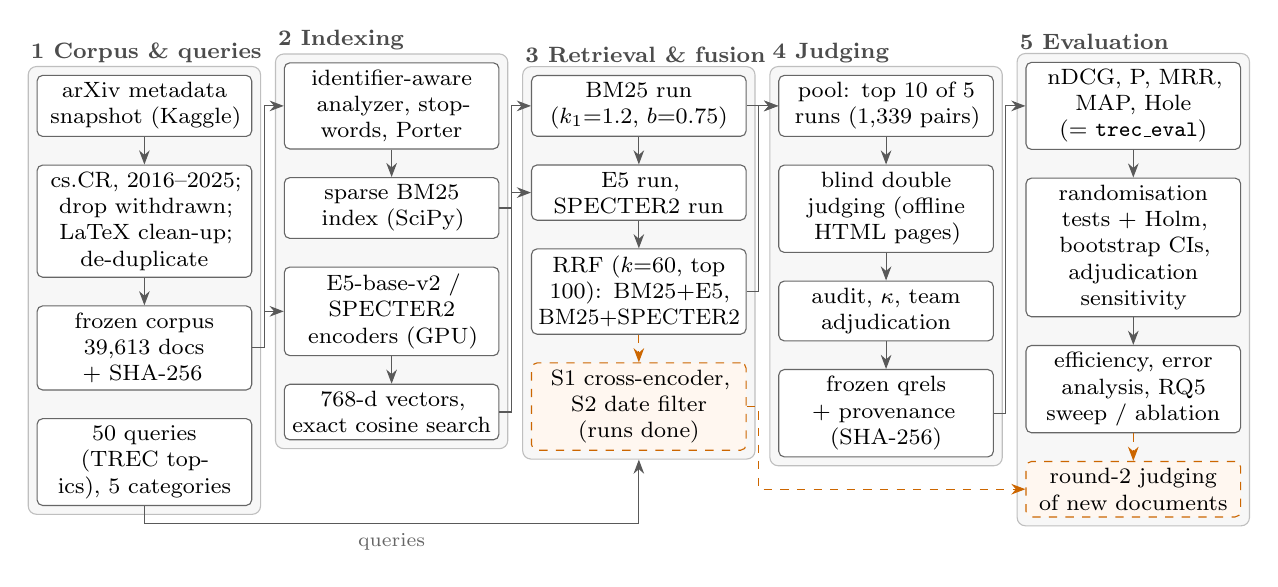
\begin{tikzpicture}[
  font=\footnotesize, node distance=3.5mm and 4mm,
  box/.style={draw=black!60, rounded corners=2pt, fill=white, align=center, inner sep=2.5pt, text width=#1},
  box/.default=2.55cm,
  todo/.style={box=#1, dashed, draw=orange!80!black, fill=orange!6},
  todo/.default=2.55cm,
  arr/.style={-{Stealth[length=1.8mm]}, black!65},
  grp/.style={draw=black!25, fill=black!3, rounded corners=3pt, inner sep=3pt},
  lab/.style={font=\footnotesize\bfseries, text=black!70, anchor=south west, inner sep=1pt}]
% column 1: data
\node[box] (snap) {arXiv metadata snapshot (Kaggle)};
\node[box, below=of snap] (clean) {cs.CR, 2016--2025; drop withdrawn; LaTeX clean-up; de-duplicate};
\node[box, below=of clean] (corp) {frozen corpus\\39{,}613 docs + SHA-256};
\node[box, below=of corp] (topics) {50 queries (TREC topics), 5 categories};
% column 2: indexing
\node[box, right=of snap] (tok) {identifier-aware analyzer, stopwords, Porter};
\node[box, below=of tok] (bmidx) {sparse BM25 index (SciPy)};
\node[box, below=of bmidx] (enc) {E5-base-v2 / SPECTER2 encoders (GPU)};
\node[box, below=of enc] (vec) {768-d vectors, exact cosine search};
% column 3: retrieval and fusion
\node[box, right=of tok] (bm) {BM25 run ($k_1$=1.2, $b$=0.75)};
\node[box, below=of bm] (dense) {E5 run, SPECTER2 run};
\node[box, below=of dense] (rrf) {RRF ($k$=60, top 100): BM25+E5, BM25+SPECTER2};
\node[todo, below=of rrf] (str) {S1 cross-encoder, S2 date filter (runs done)};
% column 4: judging
\node[box, right=of bm] (pool) {pool: top 10 of 5 runs (1{,}339 pairs)};
\node[box, below=of pool] (judge) {blind double judging (offline HTML pages)};
\node[box, below=of judge] (adj) {audit, $\kappa$, team adjudication};
\node[box, below=of adj] (qrels) {frozen qrels + provenance (SHA-256)};
% column 5: evaluation
\node[box, right=of pool] (met) {nDCG, P, MRR, MAP, Hole (= \texttt{trec\_eval})};
\node[box, below=of met] (sig) {randomisation tests + Holm, bootstrap CIs, adjudication sensitivity};
\node[box, below=of sig] (eff) {efficiency, error analysis, RQ5 sweep / ablation};
\node[todo, below=of eff] (r2) {round-2 judging of new documents};
% groups
\begin{scope}[on background layer]
\node[grp, fit=(snap)(topics)] (g1) {}; \node[grp, fit=(tok)(vec)] (g2) {};
\node[grp, fit=(bm)(str)] (g3) {}; \node[grp, fit=(pool)(qrels)] (g4) {}; \node[grp, fit=(met)(r2)] (g5) {};
\end{scope}
\node[lab] at (g1.north west) {1 Corpus \& queries}; \node[lab] at (g2.north west) {2 Indexing};
\node[lab] at (g3.north west) {3 Retrieval \& fusion}; \node[lab] at (g4.north west) {4 Judging};
\node[lab] at (g5.north west) {5 Evaluation};
% arrows
\draw[arr] (snap) -- (clean); \draw[arr] (clean) -- (corp);
\draw[arr] (tok) -- (bmidx); \draw[arr] (enc) -- (vec);
\draw[arr] (corp.east) -- ++(1.5mm,0) |- (tok.west);
\draw[arr] (corp.east) -- ++(1.5mm,0) |- (enc.west);
\draw[arr] (bmidx.east) -- ++(1.5mm,0) |- (bm.west);
\draw[arr] (vec.east) -- ++(1.5mm,0) |- (dense.west);
\draw[arr] (topics.south) -- ++(0,-2.2mm) -| node[pos=0.25, below, font=\scriptsize, text=black!60]{queries} (g3.south);
\draw[arr] (bm) -- (dense); \draw[arr] (dense) -- (rrf); \draw[arr, dashed, orange!80!black] (rrf) -- (str);
\draw[arr] (bm.east) -- (pool.west); \draw[arr] (rrf.east) -- ++(1.5mm,0) |- (pool.west);
\draw[arr] (pool) -- (judge); \draw[arr] (judge) -- (adj); \draw[arr] (adj) -- (qrels);
\draw[arr] (qrels.east) -- ++(1.5mm,0) |- (met.west);
\draw[arr] (met) -- (sig); \draw[arr] (sig) -- (eff); \draw[arr, dashed, orange!80!black] (eff) -- (r2);
\draw[arr, dashed, orange!80!black] (str.east) -- ++(1.5mm,0) |- (r2.west);
\end{tikzpicture}
\caption{System architecture as implemented. The corpus, the runs and the relevance judgments are frozen in
this order before any metric is computed. Dashed orange boxes are the remaining work.}\label{fig:arch}
\end{figure}

% ===================================================================================== page 2
\sect{IR pipeline and methodology}
\textbf{Corpus.} From one Kaggle snapshot of the arXiv metadata we keep every paper with cs.CR as primary or
cross-listed category and a first version in 2016--2025: 53{,}454 papers in the category, of which 39{,}613
remain after removing those outside the date range, 35 withdrawn papers and 12 duplicate titles. LaTeX markup
is stripped and the text is Unicode-normalised (NFKC). A document is its title plus its abstract, which fits the
512-token limit of both dense models, so no chunking is needed. The corpus is stored as JSONL with a SHA-256
checksum; the committed list of arXiv ids rebuilds it from the snapshot.

\textbf{Queries.} 50 queries, 10 per category, each in TREC format with a description and written relevance
criteria, plus 5 practice queries for annotator training. Examples: ``exploitation of Log4Shell
(CVE-2021-44228)'' (identifier), ``anonymous communication systems that are \emph{not} based on Tor''
(negation), ``copying a deployed model by repeatedly querying its prediction interface'' (paraphrase).

\textbf{Preprocessing, tokenisation and stemming.} Our analyzer lower-cases and NFKC-normalises the text and
normalises protocol versions (``TLS 1.3'', ``TLSv1.3'' $\to$ \texttt{tls1.3}). Strings that mix letters and
digits, such as \texttt{cve-2021-44228} or \texttt{sha-256}, are kept whole and never stemmed, and their parts
are indexed as well; the parts do not count towards the document length (as Lucene does for synonyms). Other
words pass through Lucene's 33 English stopwords (which include ``not'') and the Porter stemmer. A Lucene-like
analyzer without the identifier handling is kept for validation and for the ablation.

\textbf{Indexing and BM25.} We implemented BM25 ourselves on a SciPy sparse document--term matrix of raw term
frequencies (vocabulary 56{,}862 terms, 29.3\,MB), with Lucene's non-negative idf:
\[
\textstyle \mathrm{BM25}(q,d)=\sum_{t\in q}\ln\!\Big(1+\frac{N-n_t+0.5}{n_t+0.5}\Big)\cdot
\frac{f_{t,d}\,(k_1+1)}{f_{t,d}+k_1\,(1-b+b\,|d|/\mathrm{avgdl})},\qquad k_1=1.2,\; b=0.75 .
\]
For given $(k_1,b)$ the weighted matrix is computed in one vectorised step, so a query is one sparse
matrix--vector product and a parameter sweep never re-tokenises the corpus. On BEIR SciFact our BM25 is
within 0.0009 nDCG@10 of Pyserini's Lucene BM25 and shares 98\% of its top-10 documents.

\textbf{Dense retrieval.} E5-base-v2 (mean pooling, ``query:''/``passage:'' prefixes) and SPECTER2 (proximity
adapter for documents, ad-hoc query adapter for queries), both 768-dimensional and used without fine-tuning.
The corpus is encoded once on a Tesla T4 GPU (fp16) and searched exactly by cosine similarity, so no
approximate-search error can affect the comparison.

\textbf{Hybrid retrieval.} Reciprocal Rank Fusion over the top 100 of each run scores a document by
$\sum_r 1/(60+\mathrm{rank}_r(d))$, giving BM25+E5 and BM25+SPECTER2. The constant $k=60$ is fixed in advance, so nothing is tuned on our queries.

\textbf{Pooling, judging and adjudication.} The top 10 of all five runs form the pool: 1{,}339 query--document
pairs (about 27 per query). Each query was judged independently by two of the four authors on a 0--3 scale
(0 not relevant, 1 on topic but does not answer or breaks a condition, 2 relevant, 3 highly relevant), with the
six annotator pairs spread evenly. The offline judging pages show no system names or ranks, and dates only for
time queries. All 2{,}678 judgments were audited: none missing, duplicated or outside the pool. Agreement:
weighted Cohen's $\kappa=0.760$ (linear), 0.829 (quadratic), 0.795 on binary relevance (grade $\ge 2$); exact
agreement 75.7\%, above the target of $\kappa\ge0.6$ set in the proposal. The 325 conflicting pairs were resolved in a
team discussion and recorded by one member; every final grade is one of the two submitted grades. There was no
independent adjudicator, and 27 decisions rest on the title or a ``lower grade when unsure'' rule; both are
disclosed. The qrels were then frozen with a SHA-256 checksum and a provenance file that records the checksums
of the original exports, which are kept unchanged.

\textbf{Evaluation protocol.} The primary metric is nDCG@10 (gain = grade); P@5, MRR@10 and MAP@10 use grade
$\ge2$. Unjudged documents count as non-relevant and Hole@10 reports how often they occur. Our metric code
matches \texttt{trec\_eval} (via \texttt{pytrec\_eval}) on every query of every run (maximum difference
$3\times10^{-16}$). Significance: paired randomisation tests over queries (100{,}000 permutations) for all 10
system pairs with Holm--Bonferroni correction; 95\% bootstrap CIs. Because adjudication without an independent
adjudicator could sway results, we also enumerate every way of resolving the conflicts (40{,}269 per-query
combinations) and test 500 random adjudications. Per-category results (10 queries each) are exploratory.
Efficiency (index build time, index size, query latency) comes from the run logs. RQ5 sweeps 132 $(k_1,b)$
settings with 5-fold cross-validation over queries (the only tuned number we report) and compares five
analyzers at fixed $k_1, b$.

% ===================================================================================== page 3
\sect{Preliminary results}
\begin{table}[H]\centering\small
\caption{Effectiveness on the 50 cs.CR queries (frozen, adjudicated qrels) and efficiency. Hole@10 = 0 for every
system (all top-10 documents were judged). Binary metrics use grade $\ge2$. Index build: BM25 on one CPU, dense
encoding on one Tesla T4. Dense query time includes encoding the query. Hybrids: index size and build time are
the sum of their components; query time = BM25 + dense + fusion.}
\label{tab:main}
\setlength{\tabcolsep}{4.2pt}
\begin{tabular}{@{}lcccccccc@{}}
\toprule
& \multicolumn{5}{c}{Effectiveness} & \multicolumn{3}{c}{Efficiency}\\
\cmidrule(lr){2-6}\cmidrule(l){7-9}
System & nDCG@10 [95\% CI] & nDCG@5 & P@5 & MRR@10 & MAP@10 & Index (MB) & Build (s) & Query (ms)\\
\midrule
BM25 & 0.689 [0.63, 0.75] & 0.667 & 0.516 & 0.632 & 0.325 & 29.3 & 20.3 & 1.6\\
E5 & 0.713 [0.65, 0.77] & 0.693 & \textbf{0.572} & 0.693 & 0.366 & 116.0 & 174.6 & 17.3\\
SPECTER2 & 0.543 [0.47, 0.61] & 0.542 & 0.400 & 0.596 & 0.210 & 116.0 & 182.6 & 30.0\\
BM25+E5 & \textbf{0.744} [0.69, 0.80] & \textbf{0.717} & 0.560 & \textbf{0.700} & \textbf{0.369} & 145.4 & 194.9 & 19.3\\
BM25+SPECTER2 & 0.681 [0.62, 0.74] & 0.675 & 0.524 & 0.658 & 0.311 & 145.4 & 202.8 & 32.0\\
\bottomrule
\end{tabular}
\end{table}

\begin{table}[H]\centering\small
\begin{minipage}[t]{0.53\linewidth}\centering
\captionof{table}{Selected paired comparisons on nDCG@10 (randomisation test, Holm over all 10 pairs).}\label{tab:sig}
\setlength{\tabcolsep}{4pt}
\begin{tabular}{@{}lccc@{}}
\toprule
Comparison & $\Delta$ & $p_{\text{Holm}}$ & W/T/L\\
\midrule
E5 $-$ BM25 & $+$0.023 & 0.929 & 24/3/23\\
BM25+E5 $-$ BM25 & $+$0.055 & 0.023 & 32/2/16\\
BM25+E5 $-$ E5 & $+$0.031 & 0.592 & 26/2/22\\
BM25+E5 $-$ BM25+SPECTER2 & $+$0.063 & 0.031 & 29/2/19\\
BM25 $-$ SPECTER2 & $+$0.147 & 0.005 & 32/0/18\\
E5 $-$ SPECTER2 & $+$0.170 & $<$0.001 & 37/0/13\\
\bottomrule
\end{tabular}
\end{minipage}\hfill
\begin{minipage}[t]{0.44\linewidth}\centering
\captionof{table}{nDCG@10 by query category (10 queries each; exploratory).}\label{tab:cat}
\setlength{\tabcolsep}{4pt}
\begin{tabular}{@{}lccc@{}}
\toprule
Category & BM25 & E5 & BM25+E5\\
\midrule
Identifier & \textbf{0.798} & 0.662 & 0.755\\
Homonym & 0.839 & \textbf{0.846} & 0.845\\
Negation & 0.560 & \textbf{0.677} & 0.596\\
Time & 0.665 & 0.688 & \textbf{0.752}\\
Paraphrase & 0.585 & 0.692 & \textbf{0.773}\\
\bottomrule
\end{tabular}
\end{minipage}
\end{table}

\textbf{Key findings (primary experiment).}
\begin{itemize}
\item \textbf{RQ1:} E5 and BM25 are statistically indistinguishable (E5 $+$0.023, $p_{\text{Holm}}=0.93$; E5
better on 24 queries, BM25 on 23). A general dense model used without fine-tuning does not beat a careful BM25 here.
\item \textbf{RQ3:} SPECTER2 is the weakest system: significantly below BM25, E5 and both hybrids. No way of
resolving the judgment conflicts reverses these deficits.
\item \textbf{RQ4:} BM25+E5 is the best system (0.744) and significantly better than BM25 ($+$0.055,
$p_{\text{Holm}}=0.023$), but not better than E5. That advantage over BM25 is \emph{sensitive to adjudication}:
it is significant in only 7\% of 500 random adjudications, so we treat it with caution.
\item \textbf{RQ2 (exploratory):} BM25 leads on exact identifiers (0.798 vs.\ 0.662), E5 on negation (0.677 vs.\
0.560) and paraphrase (0.692 vs.\ 0.585). With 10 queries per category the CIs overlap widely.
\item \textbf{Error analysis:} every system largely ignores conditions. On negation queries 81\% of BM25's top 10
are graded 1 (60\% for E5); for ``\ldots{} \emph{not} based on Tor'', seven of BM25's top-10 titles name Tor.
Counting from first-version dates, 30--38\% of each system's top 10 on time queries breaks the date limit.
\item \textbf{Efficiency:} BM25 answers in 1.6\,ms from a 29\,MB index built in 20\,s on a CPU. The dense
indexes are 116\,MB (4$\times$) and take about 3\,min of GPU time; dense queries take 17--30\,ms. BM25+E5
costs about 12$\times$ BM25's query time for its gain.
\end{itemize}

\textbf{RQ5: BM25 sensitivity (exploratory).} Run on the real corpus after three checks (frozen qrels
checksum, corpus checksum, and exact reproduction of the pooled BM25 run). Near the default BM25 is flat: no
setting of the 132 beats $k_1$=1.2, $b$=0.75 on nDCG@10, 12 lie within 0.01, and 5-fold cross-validated tuning
gives no gain (0.684 vs.\ 0.689). Replacing our identifier-aware analyzer with the Lucene-like one changes
nDCG@10 by only $-$0.003 ($p_{\text{Holm}}=0.27$; 41 of 50 queries unchanged), a comparison almost unaffected by
missing judgments. \emph{Limitation:} only the default BM25 run was pooled, so settings far from it, and the
analyzers without stemming or without stopword removal, retrieve documents nobody judged (up to 30\% of the top 10
for $k_1$/$b$ settings and 24\% for the analyzers). For
stemming, ordinary nDCG@10 ($-$0.089 without stemming) and nDCG@10 computed on judged documents only
($+$0.033) point in opposite directions, so that question stays open until the documents are judged
(Section~\ref{sec:plan}).

% ===================================================================================== page 4
\sect{Contribution matrix}
\begin{table}[H]\centering\small
\caption{Contributions. The judgment counts come from the committed judgment exports. The responsibility areas
are the group's \emph{proposed} allocation and are to be confirmed by all four members before submission;
commits are made under a shared group identity, so the repository does not record individual authorship.}
\label{tab:contrib}
\begin{tabularx}{\linewidth}{@{}>{\raggedright\arraybackslash}p{2.75cm} >{\raggedright\arraybackslash}X >{\raggedright\arraybackslash}p{4.3cm}@{}}
\toprule
Member & Responsibility area (proposed; to be confirmed) & Recorded in the repository\\
\midrule
Surajsinh Patil\newline 2025H1030058P & Query formulation; relevance-judgment workflow; annotation agreement analysis; retrieval error analysis & 672 relevance judgments; recorded the team's adjudication decisions\\
Tejas Mahajan\newline 2025H1030057P & Dense retrieval experiments (E5, SPECTER2); embedding-based retrieval analysis; evaluation comparisons & 674 relevance judgments\\
Swayam Kumud\newline 2025H1030063P & BM25 implementation and indexing; experiment integration; evaluation pipeline; report coordination & 635 relevance judgments\\
Saksham Singhal\newline 2025H1030208P & Corpus preprocessing; tokenisation analysis; experimental validation; result visualisation & 697 relevance judgments\\
\bottomrule
\end{tabularx}
\end{table}
All four members judged relevance (2{,}678 judgments in total, every query by two members) and took part in the
team discussion that resolved the 325 judgment conflicts.

\sect{Remaining work (about 20--25\%) and plan to the final submission}\label{sec:plan}
The core experiments are complete and frozen; we do not plan to re-run or re-judge them. The remaining work
extends the evaluation to the systems that were not in the original pool, which is also where our stretch
objectives sit. The original qrels stay frozen: new judgments go into a separate, versioned extension with its
own checksum and provenance, and every result will say which qrels it uses.

\begin{table}[H]\centering\small
\caption{Remaining work packages. ``Lead'' follows the proposed responsibility areas and is to be confirmed.}\label{tab:plan}
\renewcommand{\arraystretch}{1.25}
\begin{tabularx}{\linewidth}{@{}>{\raggedright\arraybackslash}p{3.6cm} >{\raggedright\arraybackslash}X >{\raggedright\arraybackslash}p{2.3cm}@{}}
\toprule
Work package (status now) & Final deliverable & Lead (proposed)\\
\midrule
\textbf{W1} Round-2 blind judging (not started; pairs identified) & 272 unjudged top-10 query--document pairs on 48 queries (from S1, S2 and the RQ5 variants), judged by two members each with the same pages and guide; $\kappa$, adjudication, extended qrels frozen with checksum & all members; workflow: Surajsinh Patil\\
\textbf{W2} S1 cross-encoder re-ranking (run done; 28\% of its top 10 unjudged) & nDCG@10 and significance against BM25+E5 on the extended qrels; per-category effect, testing the expectation that it helps negation queries most & Tejas Mahajan\\
\textbf{W3} S2 date filter (run done; rule-based date extraction, 3\% unjudged) & Effect on the time category and on the share of date violations (30--38\% today); LLM-based date extraction only if time allows & Saksham Singhal\\
\textbf{W4} S4 tuned score fusion; S3 LLM judge (code done, not run on cs.CR) & S4: convex score combination tuned by 5-fold CV vs.\ RRF. S3 (optional, needs API access): LLM vs.\ human $\kappa$ and Kendall's $\tau$ of the system ranking & Swayam Kumud (S4); Tejas Mahajan (S3)\\
\textbf{W5} RQ5 completion and pool-bias analysis & Stemming and stopword ablation re-scored on the extended qrels; how much scores of non-pooled runs change once their documents are judged & Saksham Singhal\\
\textbf{W6} Final report, reproducibility and demo & Error analysis for the new runs; fresh end-to-end Kaggle re-run from a tagged commit; release of queries, qrels, runs and code; presentation and live demo of the judging pages and retrieval; confirmed contribution matrix & Swayam Kumud (report); Surajsinh Patil (error analysis); all\\
\bottomrule
\end{tabularx}
\end{table}

\textbf{Success criteria from the proposal.} All four are met: (i)~our BM25 is within 0.01 nDCG@10 of Pyserini on
BEIR SciFact ($-$0.0009); (ii)~our metric code gives the same numbers as \texttt{pytrec\_eval}; (iii)~weighted
$\kappa\ge0.6$ (0.760); (iv)~every conclusion is backed by a corrected significance test or marked exploratory.

\textbf{Deviations from the proposal.} (1)~The filtered collection has 39{,}613 documents, fewer than the planned
cap of 50{,}000, so it is used in full rather than sampled. (2)~S2 extracts date ranges with rules, which parse
all 10 time queries, instead of an LLM. (3)~Conflicts were resolved in a team discussion rather than by an
independent adjudicator; we disclose this and report how sensitive each comparison is to it.

\textbf{Order and risks.} W1 comes first because W2, W3 and W5 depend on it. At two judgments per pair, W1 is
544 judgments, about 136 per member, roughly a fifth of round 1. If time runs short we drop W4's optional S3
part before anything else, and report any stretch result whose judgments are incomplete as preliminary with
its Hole@10.

\textbf{Expected final deliverables.} (1)~Final report with all five research questions and the evaluated
stretch objectives; (2)~the cs.CR test collection: 50 queries, original and extended qrels with provenance,
all run files; (3)~the code repository with tests, Kaggle notebooks and a one-command evaluation pipeline;
(4)~presentation and demonstration.

\end{document}
